\chapter{Introduction}
\label{chap:introduction}
For robots it remains a hard problem to navigate and act in new, unseen environments. Most approaches controlling the robot and acting as the robot brain fall in one of two categories. The bulk falls into hierarchical approaches~\cite{kaelbling_hierarchical_2011,scholz_navigation_2016,krontiris_dealing_2015}, an hierarchical structure generally consists of an high-level and low-level component. The high-level task planner tries to understand and model the environment, suck gained knowledge is used to generate action sequences toward a desired goal. The high-level planner sends actions to a low-level module, that takes care of sending input signals toward the robot actuators. The high-level planner has a prediction horizon consisting of an action sequence, a long prediction horizon compared to the low-level planner which prediction horizon is maximal one action. Hierarchical structures genarally provide solutions which are computationally effecient but are hierarchical solutions, meaning the solutions found are are teh best feasible solutions in the task hierarchy they search. The quality of the solution depends on the hierarchy which are typically hand-coded and domain specific~\cite{vega-brown_asymptotically_2020}. Altanively to hierarchical approaches, solutions can be provided by searching in a joint configuration space of the robot and obstacles, where the robots configuration space is augmented with environment obstacles configuration spaces whilst also including dynamic constraints~\cite{hauser_multimodal_2010,berenson_manipulation_2009,jaillet_path_2013}. Such a joint configuration space suffers from a combinational explosion and is practically impossible to search. Finding an action sequence from searching in a joint configuration is exaustive, instead for example a search close to the the current configuration, let the robot track this incomplete solution toward a desired goal and search the joint configuration space again close to the new current configuration. different techniques exist to prevent searching in the entire joint configuration space.\bs

Robots in new unforeseen environments is a broad topic, let's narrow down the scope. The focus lies on the challenging and largely unsolved problem of navigation among movable obstacles in unknown environments. Consider a simple robot without grippers or arms attached in an environements with movable obstacles. By sending input toward the wheels the robot can drive around. The environment consists of a flat ground plane, the robot and movable obstacles which the robot can manipulate by pushing. This creates two different modes of dynamics (driving, pushing) different differential constraints apply to the different modes, the different modes of dynamics result in a piecewise-analytic configuration space which hardens motion planning considerably~\cite{vega-brown_asymptotically_2020}. Whilst the robot can interact with the obstacles in the environment, there is no prior information provided to the robot (e.g. weight, friction coefficient) other than the shape and pose of the obstacle. By interaction with obstacles the robot can generate a system model, describing the expected trajactory of an obstacle as result of a push from the robot. The robot is tasked to relocate a subset of obstacles by means of pushing obstacles. \bs

Applicable to such an robot environment three topics in robotics investigated, these topics are \textbf{motion planning}, \textbf{non-prehensile manipulation planning}, and \textbf{learning obstacle dynamics}. Whilst individually a considerable amount of research is done in these topics (motion planning~\cite{lavalle_planning_2006,elbanhawi_samplingbased_2014,kingston_samplingbased_2018,chen_fast_2018}, pusing obstacles to target locations~\cite{arruda_uncertainty_2017,mericli_pushmanipulation_2015,toussaint_sequenceofconstraints_2022,stuber_let_2020,stuber_featurebased_2018,bauza_dataefficient_2018}, learning obstacle dynamics~\cite{seegmiller_vehicle_2013,cong_selfadapting_2020}), combining 2 out of these 3 topics is lesser researched and combining all three even scarcer.\bs

\citeauthor{vega-brown_asymptotically_2020} investigated motion planning in a piecewise-analytic configuration space to relocate obstacles~\cite{vega-brown_asymptotically_2020}. Whilst an an optimal plan is obtained with probability one with infinite samples, the algorithm does not learn the pushing relation between the robot and the obstacles. The ability to learn push dynamics greatly broadens the variety of obstacles a robot can push. Realisticly robots in warehouses, hospitals or supermarkets might encounter a variety of different obstacles, but learning dynamics inavitably leads to system model mismatch. An motion planning algorithm should be competable with learned system models and take model mismatch into account.\bs

\citeauthor{wang_affordancebased_2020} takes pushing objects to target location out of the equation and only focussus on the \ac{NAMO} problem. Learning interaction by embedding unknown obstacles with affordance information followed by planning with a contact-implicit motion planner toward a robot goal location~\cite{wang_affordancebased_2020}. By removing pushing obstacles finding a path from start to target configuration simplifies, the piecewise-analytic configuration spaces becomes a configuration space. There exist a variety of sampling-based motion planners that can find a path with properties such as probabilistic completeness, replanning in dynamic environments, planning under uncertainty or asymtotically optimality~\cite{karaman_samplingbased_2011,elbanhawi_samplingbased_2014}.\bs

\citeauthor{vega-brown_asymptotically_2020} combines \ac{NAMO} with non-prehensile manipulation panning, \citeauthor{wang_affordancebased_2020} combines \ac{NAMO} with learning system models. both combine 2 of the 3 topics allowing for an more in depth analysis but avoiding the problems introduced by combining all 3 topics (\ac{NAMO}, non-prehensile manipulation plannning and learning system models). \citeauthor{sabbaghnovin_model_2021} does combine all three topics. She proposes to obtain system models by analysing and converting a limited set of robot-obstacle test pushes using Bayesian regression to predict model parameters. Path planning is the result of solving an proposed mixed-integer convex optimization~\cite{sabbaghnovin_optimal_2016} which is tracked by \ac{MPC} control, the proposed method is tested in a hospital setting~\cite{novin_dynamic_2018} and was later improved upon resulting in lowering trajectory errors~\cite{sabbaghnovin_model_2021}.\bs

Since \citeauthor{sabbaghnovin_model_2021} uses a gripper to manipulate obstacles, the reseach falls into the category prehensile manipulation. Prehensile manipulation in comparinson with non-prehensile manipulation is simpler because a pushed obstacle becomes disconnected easier compared to a gripped obstacle. Research from~\cite{novin_dynamic_2018,sabbaghnovin_model_2021} is specific to legged obstacles, which limits the set of obstacles to manipulate considerably.\bs

This thesis proposes a method where the robot should learn robot and obstacle dynamics by interaction, perform motion and manipulation planning whilst facing a wide variety of obstacles, tasks and environments. The 3 topics (\ac{NAMO}, non-prehensile manipulation plannning and learning system models) are bundled together with a technique known as \textbf{backward induction} also known as \textbf{backward tracing} or \textbf{backward search} (this thesis will refer to this technique with the term backward search). The proposed method in this thesis and \citeauthor{sabbaghnovin_model_2021} proposed method solve comparible problems using different techniques, allowing for easy comparinson between the the results of \citeauthor{sabbaghnovin_model_2021} and the results from the proposed method in this thesis.\bs

\section{Report Structure}
\todo[inline]{Create the report structure when the report structure does not change any more}

\section{Research Question}
\textbf{Main research question:}
\begin{center}
\label{researchquestion:main}
\large
How do obstacles' system models learned by a nonprehensile manipulation robot during\\  task execution improve global task planning?
\end{center} 

\textbf{Research subquestion:}
\begin{enumerate}
    \item\label{researchsubquestion:does_it_work} How does backtracing~\cite{krontiris_dealing_2015} while remembering interactions with unknown obstacles compare to not remembering learning interactions over time?
    \item\label{researchsubquestion:does_it_compare} Can the proposed method combine learning and planning for push en drive applications? Can the proposed method complete tasks, and how does it compare against the state of the art? 
\end{enumerate}

\todo[inline]{why these researchs questions, eleborate a bit more on them}

\section{Problem Description}
\label{sec:problem_description}
Tests are performed in a robot simulation environment, let's start with defining the environment.\\Let the tuple $\left\langle \text{Origin}, \text{Ground Plane}, \text{Ob}, E \right\rangle$ fully define a robot environment where:\bs

\par\smallskip\noindent
\centerline{\begin{minipage}{0.8\textwidth}
\begin{enumerate}
  \item[Origin] Static point in the environment with a $x$-, $y$- and $z$-axis. Any point in the environment has a linear and an angular position and velocity with respect to the origin \vspace{0.5\baselineskip}
 \item[Ground Plane] A flat plane parallel with the Origin's $x$- and $y$- axis. Obstacles cannot pass through the ground plane and meet sliding friction when sliding over the ground plane. \vspace{0.5\baselineskip}
 \item[Ob] A set of obstacles, $\text{Ob} = (obst_1, obst_2, obst_3, \dots, obst_i)$ with $i>1$, an obstacle is an 3-dimensional body with shape and uniformly destributed mass. Examples of obstacles are given in \cref{fig:example_obstacles}. \vspace{0.5\baselineskip}
  \item[$E$] A set of motion equation describing the behaviour of obstacles such as gravity, interacteraction with the ground plane or interaction with other obstacles. The motion equations are equivalent to the true dynamics. \vspace{0.5\baselineskip}
\end{enumerate}
\end{minipage}}
\par\smallskip

A state consists of the linear and angular position and velocity of a point with respect to the environment's origin.\bs
Formally, a \textbf{state}, $s_{id}(k)$ is a tuple of $\left\langle pos_x(k), pos_y(k), pos_\theta(k), vel_x(k), vel_y(k), vel_\theta(k)\right\rangle$\\ where $pos_x, pos_y, vel_x, vel_y, vel_\theta \in \mathbb{R}, \quad  pos_\theta \in [0, 2\pi)$.\\

\subsection{Task}
\label{subsec:task}
The task is defined as a subset of obstacles with target positions:\bs
$$\text{task} = \left\langle Ob_{task}, S_{target} \right\rangle$$

where $Ob_{task} = (obst_1, obst_2, obst_3, \dots, obst_k) \subset Ob$, $S_{target} = (s_1, s_2, s_3, \dots s_k)$ and $k>0$

\subsection{Assumptions}
\label{subsec:assumptions}
In order to simplify the pushing and learning problem, a number of assumptions are taken, which are now listed.\bs

\begin{assumption*}
\label{assumption:closed_world}
\textbf{Closed-World Assumption:} Objects are manipulated, directly or indirectly only by the robot. Objects cannot be manipulated by influences from outside the environment.
\end{assumption*}\bs

\begin{assumption*}
\label{assumption:quasi_static}
\textbf{Quasi-Static Assumption:} Velocities are small enough that inertial forces are negligible~\cite{stuber_let_2020}.
\end{assumption*}\bs

\begin{assumption*}
\label{assumption:perfect_obstacle_sensor}
\textbf{Perfect Obstacle Sensor Assumption:} the robot has full access to the poses and geometry of all obstacles in the environment at all times.
\end{assumption*}\bs

\begin{assumption*}
\label{assumption:order_does_not_matter}
\textbf{Tasks are Commutative Assumption:} Tasks exist of multiple obstacles with specified target positions. The order in which obstacles are pushed toward their target position is commutative.
\end{assumption*}\bs

\begin{assumption*}
\label{assumption:no_tipping}
\textbf{Obstacles do not tip over Assumption:} Movable obstacles slide if pushed.
\end{assumption*}\bs

The assumptions taken serve to simplify the problem of task completion. Note that in \cref{sec:future_work} insight is given to remove all but Assumption 2. By removing assumptions completing tasks becomes a harder problem, but a more realistic problem closer to the real world applications.\bs

Assumptions might have certain implications, which are now listed. The \hyperref[assumption:closed_world]{\textbf{closed-world assumption}} implies that obstacles untouched by the robot and with zero velocity component remain at the same position. Completed subtasks are therefore assumed to be completed for all times after completion time.\bs

The \hyperref[assumption:quasi_static]{\textbf{quasi-static assumption}} allows to neglect complex dynamics, which in many cases are negligible. To ensure that complex dynamics do not become significant during testing, a maximum robot speed or accelaration is enforced.\bs

The \hyperref[assumption:perfect_obstacle_sensor]{\textbf{perfect obstacle sensor assumption}} simplifies a sensor setup, it prevents Lidar-, camera setups and for tracking setups with aruco or other motion caputer markers. The existence of a single perferct measurement wipes away the need to combine measurements from multiple sources with sensor fusion algorithms, such as Kalman filtering \cite{verhaegen_filtering_2007}.\bs

Certain tasks are only feasible if performed in a certain order (e.g. the Tower of Hanoi), the \hyperref[assumption:order_does_not_matter]{\textbf{tasks are commutative assumption}} allows to focus only on a single subtask since it does not affect the completion or feasibility of other subtasks.\bs

The \hyperref[assumption:no_tipping]{\textbf{obstacles do not tip over assumption}} ensures that obstacles do not tip over and suddenly have vastly different dynamics. In practice obstacles will not be higher than the minimum width of the obstacle, and spheres are excluded since rolling essentially is tipping. 

\subsection{Robot Environment Example}

\begin{figure}[H]
    \centering
    \begin{subfigure}{.5\textwidth}
    \centering
    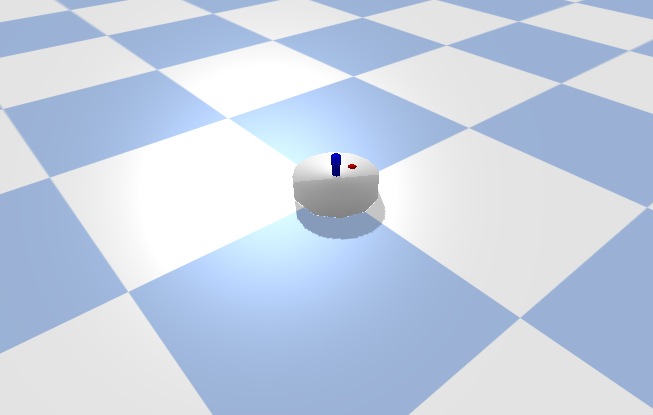
\includegraphics[width=0.8\textwidth]{figures/point_robot.png}
    \caption{The holonomic point robot\\the 2 inputs drive the robot in $x$ and in $y$ direction}
    \label{subfig:example_point_robot}
    \end{subfigure}%
    \begin{subfigure}{.5\textwidth}
    \centering
    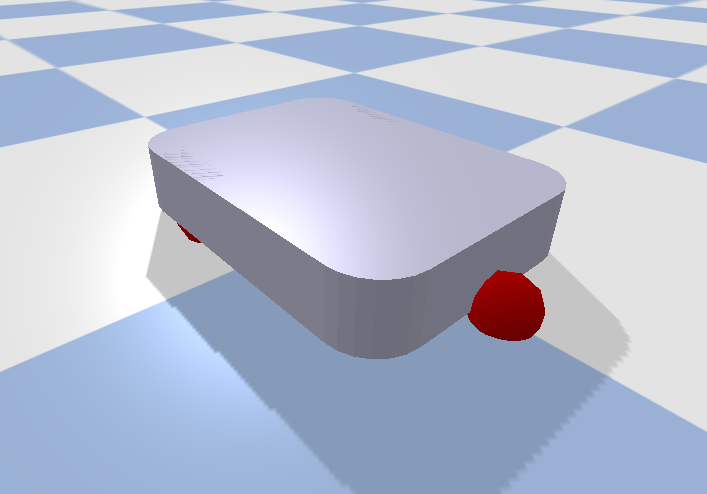
\includegraphics[width=0.8\textwidth]{figures/boxer_robot.png}
    \caption{The nonholonomic boxer robot\\the first input drives the robot forward/backward\\the second rotates the robot}
    \label{subfig:example_boxer_robot}
    \end{subfigure}%
    \caption{Robots used for testing, for either robot an velocity and a accelaration input exists, in total 4 different robots are used}
    \label{fig:example_robots}
\end{figure}
\todo[inline]{zoom in a bit on these 2 cute robots}

\begin{figure}[H]
    \centering
    \begin{subfigure}{.5\textwidth}
    \centering
    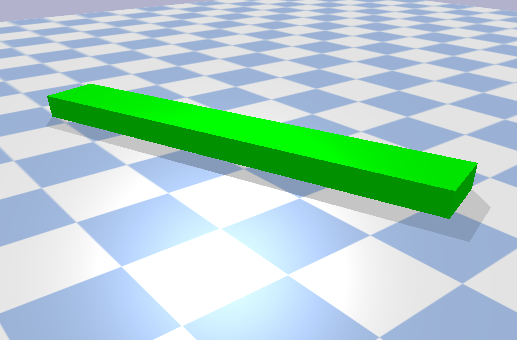
\includegraphics[width=0.8\textwidth]{figures/box_obstacle.png}
    \caption{A box obstacle}
    \end{subfigure}%
    \begin{subfigure}{.5\textwidth}
    \centering
    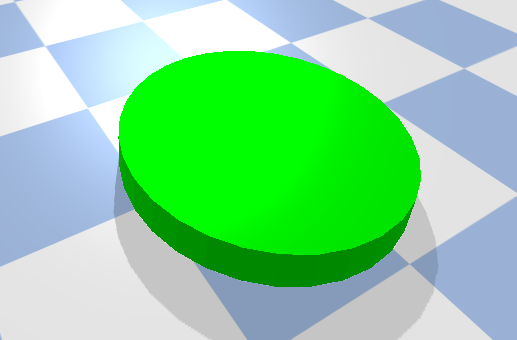
\includegraphics[width=0.8\textwidth]{figures/cylinder_obstacle.png}
    \caption{A cylinder obstacle}
    \end{subfigure}%
    \caption{Various obstacles in the robot environment}
    \label{fig:example_obstacles}
\end{figure}

\todo[inline]{introduce the exmaple env plaeze}

\subsection{Arisen Problems}
\label{subsection:problems_with_task_planning}
Assuming the task has at least a one obstacle to place at a target state (exclude purely \ac{NAMO} problems), finding an optimal solution to a task is \ac{NP-hard} since, it can be reduced to the piano mover's problem which is known to be \ac{NP-hard}~\cite{reif_motion_1985}.\\Problems in class P have an solution which can be found in polynomial time, problems in ac{NP} are problems for which a solution cannot found in polynomial time. For problems in \ac{NP}, when provided with a solution, verifying that the solution is indeed an valid solution can be done in polynomial time. \ac{NP-hard} problems are a class of problems which are at least as hard as the hardest problems in \ac{NP}. Problems that are \ac{NP-hard} do not have to be elements of NP. They may not even be decidable~\cite{pokharel_computational_2020}.\\This thesis, or other recent studies in the references do not attempt to find an optimal solution. Instead they provide a solution whilst guaranteeing properties such as near-optimality or probabilistic completeness.\bs 

Finding a solution to a task requires a search in the \textit{joint configuration space} which comes with 2 problems to tackle. Before investigating a problem, let's investigate how to construct a joint configuration space which is created by augmenting the robot's configuration space with the configuration space of every obstacle. For example, if the configuration space for both robot and obstacles consist of position $x$, $y$ and orientation $\theta$, then the joint configuration space is $3n$-dimensional, where $n$ is the number of obstacles including the robot. the joint configuration space's dimensionality grows linearly, meaning the joint configuration space grows exponentially in the number of obstacles, which is an explosion in the number of possible combinations the environment can be in, this is the first problem with a joint configuration space.\\Unspecified target positions are a fine example of the curse of dimensionality, consider a blocked corridor. The obstacle needs to be pushed to free the path but the target location of this obstacle is unspecified, as long as the robot can drive through the corridor unhindered. A solution is, the robot drives to the obstacle, pushes the obstacle, and then drives through the corridor. The push action influences the free space where the robot has to drive in when the push action was completed. Even sampling-based search algorithms cannot computationally find a path between a start en target state in joint configuration space in reasonable time (orders of magnitude slower than real-time).\\Only by leveraging simplifications of the joint configuration space a search be performed, such as discretization~\cite{sabbaghnovin_optimal_2016}, factorization~\cite{vega-brown_asymptotically_2020} or a heuristic function combined with a time horizon~\cite{sabbaghnovin_optimal_2016}. Such techniques prevent searching in configurations relatively far from the current configuration, while optimality guarantees can be given and real-time implementations have been shown.\bs

The second problem is that the joint configuration space is \textit{piecewise-analytic}. Let's eleborate, when the robot drives constraints apply due to e.g. the robot being nonholonomic. When the robot pushes an obstacle a different set of constraints are applicable, creating 2 different modes of dynamics. A configuration space containing multiple modes of dynamics is an piecewise-analytic configuration space~\cite{vega-brown_asymptotically_2020}. Motion planners have great difficulty with crossing the boundary from one mode of dynamics to another.




